% Built on the SSY340 poster template: https://github.com/dml-cth/deep-machine-learning/tree/master/poster-template
% (adapted from https://github.com/deselaers/latex-beamerposter/blob/master/examples/03/poster.tex)


\documentclass{beamer}
\usepackage[orientation=portrait,size=a2,scale=1.3,debug]{beamerposter}
\mode<presentation>{\usetheme{ZH}}
\usepackage[utf8]{inputenc}
\usepackage[english]{babel}
\usepackage{siunitx} %pretty measurement unit rendering
\usepackage{hyperref} %enable hyperlink for urls
\usepackage{ragged2e}
\usepackage{multicol}
\usepackage[font=scriptsize,justification=justified]{caption}
\usepackage{array,booktabs,tabularx}
\usepackage{amsmath}
\usepackage{tikz}
\usetikzlibrary{positioning,arrows.meta,calc}

% Replacement font for Akzidenz
\usepackage{helvet}

\newcolumntype{Z}{>{\centering\arraybackslash}X} % centered tabularx columns

% Same colours as the figures: real / clean vs crafted / attacked
\definecolor{cleanC}{HTML}{2563B0}
\definecolor{attackC}{HTML}{EB6834}
\definecolor{truthC}{HTML}{2E8B57}
\definecolor{predC}{HTML}{D62728}
\definecolor{laneC}{HTML}{C4A35A}
\newcommand{\stat}[1]{{\Large\bfseries\color{attackC}#1}}

% One line per reference instead of author / title / venue on separate lines
\setbeamertemplate{bibliography entry title}{}
\setbeamertemplate{bibliography entry location}{}
\setbeamertemplate{bibliography entry note}{}

% Top view of a car heading +x, centred at (#1, #2), labelled #3
\newcommand{\topcar}[3]{%
	\begin{scope}[shift={(#1, #2)}]
		\draw[fill=white, line width=1.2pt, rounded corners=5pt] (-0.8, -0.36) rectangle (0.8, 0.36);
		\fill[black!55, rounded corners=2pt] (0.22, -0.28) rectangle (0.48, 0.28);
		\fill[black!55, rounded corners=2pt] (-0.68, -0.25) rectangle (-0.52, 0.25);
		\node[font=\footnotesize\bfseries] at (-0.15, 0) {#3};
	\end{scope}}

% Layer slab in oblique view (thin front face, side face, top) named #1: flow line at (#2, #3), height #4, fill #5
\newcommand{\slab}[5]{%
	\colorlet{slabC}{#5}%
	\pgfmathsetmacro{\slabB}{#3 - #4/2 - 0.17}%
	\filldraw[fill=slabC, draw=black!70, line width=0.5pt] (#2+0.05, \slabB) -- ++(0.3, 0.34) -- ++(0, #4) -- ++(-0.3, -0.34) -- cycle;
	\filldraw[fill=slabC!55!white, draw=black!70, line width=0.5pt] (#2-0.05, \slabB+#4) -- ++(0.1, 0) -- ++(0.3, 0.34) -- ++(-0.1, 0) -- cycle;
	\filldraw[fill=slabC!75!white, draw=black!70, line width=0.5pt] (#2-0.05, \slabB) rectangle ++(0.1, #4);
	\coordinate (#1-in) at (#2-0.05, #3);
	\coordinate (#1-out) at (#2+0.35, #3);
}

\title{\huge Adversarial Attack on\\[0.3ex]Multimodal Trajectory Prediction}
\author{Group 33: Kaushik Rathnakar Shetty, Yanran Xie}
\institute[Chalmers]{Chalmers University of Technology}
\date{\today}
\newcommand{\posteremail}{\href{mailto:kaushikr@chalmers.se}{kaushikr@chalmers.se}, \href{mailto:yanra@student.chalmers.se}{yanra@student.chalmers.se}}

% edit this depending on how tall your header is.
\newlength{\columnheight}
\setlength{\columnheight}{51cm}


\begin{document}
\begin{frame}
\vspace*{0.8cm}
\begin{columns}
	\begin{column}{.43\textwidth}
		\begin{beamercolorbox}[center]{postercolumn}
			\begin{minipage}{.98\textwidth}  % tweaks the width, makes a new \textwidth
				\parbox[t][\columnheight]{\textwidth}{
					\begin{myblock}{Motivation: can 18\,cm of driving fool a predictor?}
						\noindent Self-driving cars act on where they predict others will go, and an attacker controls one input: \textbf{its own path}. Following Zhang et al.~\cite{zhang2022adversarial}, we attack our map-aware GNN predictor: how vulnerable is it, which part resists, and why?
						\begin{figure}
							\centering
							\begin{tikzpicture}[font=\small, line cap=round,
								road/.style={laneC, line width=1.5pt, dash pattern=on 10pt off 7pt},
								dot/.style={circle, fill, inner sep=2.2pt},
								lab/.style={font=\small\bfseries, inner sep=1pt}]
								% two lanes, 1.45 cm wide: the predicted car on top, the predicting car below
								\foreach \oy/\title/\attacked in {0/Without attack/0, -3.75/With attack/1} {
									\begin{scope}[yshift=\oy cm]
										\foreach \y in {0, 1.45, 2.9}
											\draw[road] (0, \y) -- (14.4, \y);
										\node[anchor=south west, lab, inner sep=0] at (0, 3.08) {\title};
										\ifnum\attacked=0
											\draw[cleanC, line width=2.5pt] (0.5, 2.175) -- (4.4, 2.175);
											\foreach \x in {0.5, 1.48, 2.45, 3.43} \node[dot, cleanC] at (\x, 2.175) {};
											\node[cleanC, anchor=south, lab] at (2.2, 2.25) {real past};
											\draw[predC, line width=2.5pt, dash pattern=on 8pt off 5pt] (6.0, 2.08) -- (14.0, 2.04);
											\node[predC, anchor=north, lab] at (11.6, 1.98) {prediction};
											\node[anchor=west, font=\small] at (3.7, 0.725) {keeps its speed};
										\else
											\draw[attackC, line width=2.5pt] plot[smooth] coordinates {(0.5, 2.03) (1.48, 2.32) (2.45, 2.06) (3.43, 2.3) (4.4, 2.175)};
											\foreach \x/\y in {0.5/2.03, 1.48/2.32, 2.45/2.06, 3.43/2.3} \node[dot, attackC] at (\x, \y) {};
											\node[attackC, anchor=south, lab] at (2.2, 2.36) {crafted past};
											\draw[predC, line width=2.5pt, dash pattern=on 8pt off 5pt] (6.0, 2.12) .. controls (9.0, 2.12) and (10.6, 0.88) .. (14.0, 0.85);
											\node[predC, anchor=north east, lab] at (14.0, 0.62) {prediction};
											\node[anchor=west, lab, predC, font=\small\bfseries\itshape] at (3.7, 0.725) {cut-in?\ brake!};
										\fi
										\draw[truthC, line width=2.5pt] (6.0, 2.24) -- (14.0, 2.24);
										\node[truthC, anchor=south, lab] at (11.6, 2.3) {true future};
										\topcar{5.2}{2.175}{}
										\topcar{2.6}{0.725}{}
									\end{scope}
								}
							\end{tikzpicture}
							\caption{After~\cite{zhang2022adversarial}. The lower car predicts the upper car's path (red) and brakes for a cut-in that never comes.}
						\end{figure}
						\vspace{-0.5cm}
					\end{myblock}\vfill
					\begin{myblock}{Example: 15\,cm per point forces a right turn}
						\begin{figure}
							\centering
							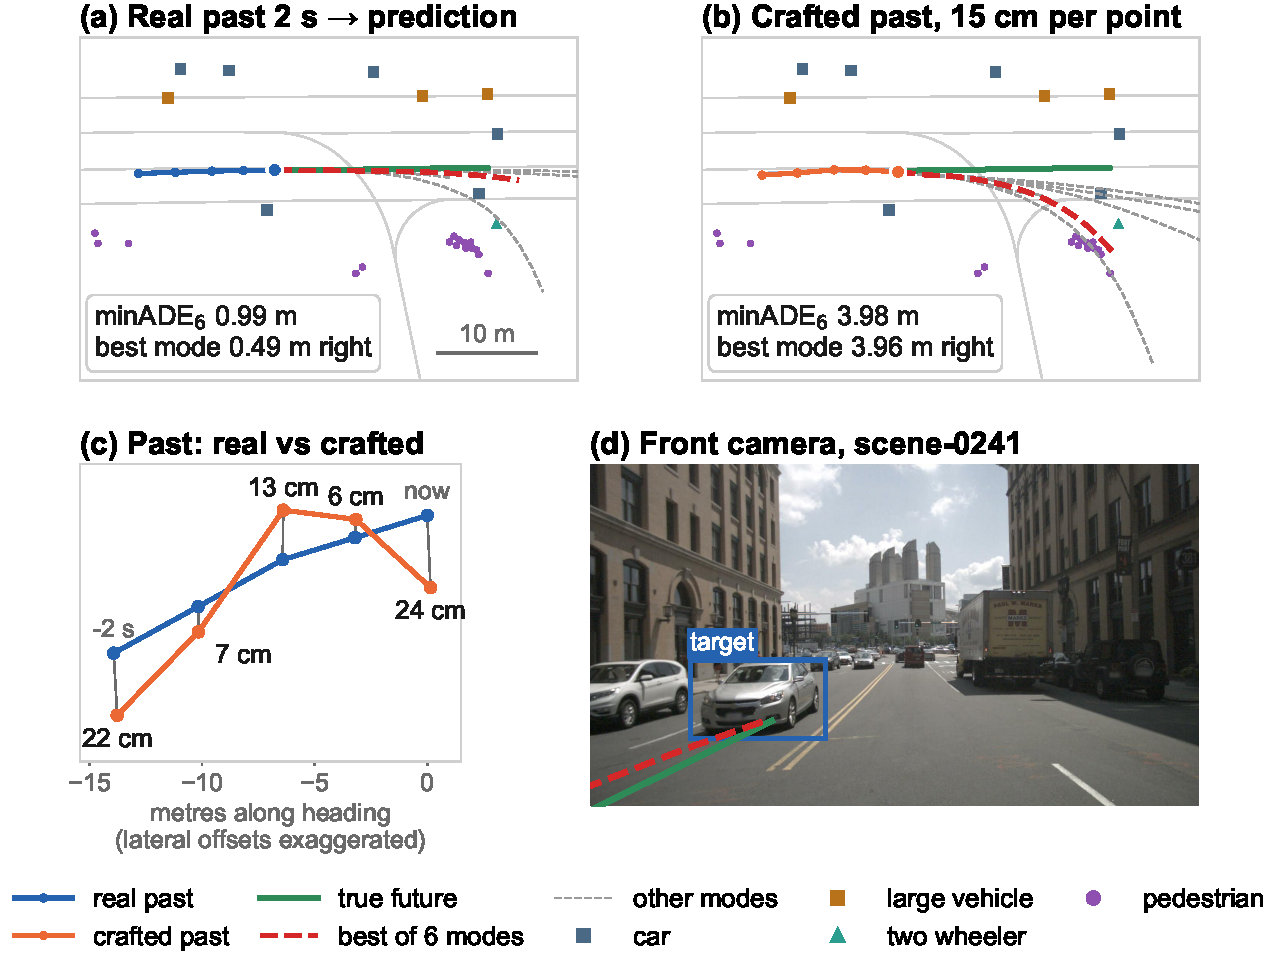
\includegraphics[width=\linewidth]{figures/hero_example.pdf}
							\caption{Final model (seed 42), nuScenes~\cite{caesar2020nuscenes} scene-0241. Chosen for clarity: for this seed, the right attack crosses half a lane in 21.6\% of samples.}\label{fig:example}
						\end{figure}
					\end{myblock}\vfill
					\begin{myblock}{Why is our model so easy to fool?}
						% each reason on the left, its evidence on the same row to the right
						\noindent\begin{minipage}[c]{0.52\linewidth}
							\raggedright\textbf{1. Short history, long horizon.} Speed is read from 5 past points, so a shift grows over the 6\,s forecast. Even constant velocity, which learns nothing, adds 21\,m per metre of shift (ours: 7\,m).
						\end{minipage}\hfill
						\begin{minipage}[c]{0.4\linewidth}
							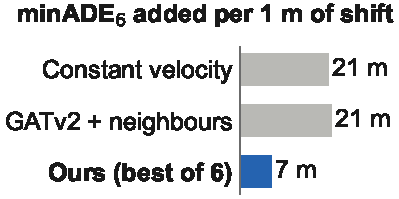
\includegraphics[width=\linewidth]{figures/why_amplification.pdf}
						\end{minipage}
						\par\vspace{0.5cm}
						\noindent\begin{minipage}[c]{0.52\linewidth}
							\raggedright\textbf{2. It trusts only what the attacker controls.} Without the target's motion the error rises by 6.5\,m, without neighbours by only ${\approx}0.001$\,m: no other input can contradict a faked past.
						\end{minipage}\hfill
						\begin{minipage}[c]{0.4\linewidth}
							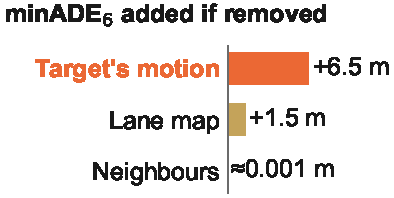
\includegraphics[width=\linewidth]{figures/why_inputs.pdf}
						\end{minipage}
						\par\vspace{0.5cm}
						\noindent\begin{minipage}[c]{0.52\linewidth}
							\raggedright\textbf{3. Six modes move together.} They share one context, so the whole fan shifts: under the ADE attack, samples with no mode within 2\,m rise from 63\% to 96\%.
						\end{minipage}\hfill
						\begin{minipage}[c]{0.4\linewidth}
							\resizebox{\linewidth}{!}{%
							\begin{tikzpicture}[line cap=round, font=\small, dot/.style={circle, fill, inner sep=2pt}]
								% six modes before the attack (faint), around the truth
								\foreach \e in {1.2, 0.9, 0.6, 0.3, 0.0, -0.3}
									\draw[black!15, line width=1.6pt] (2.95, 0) .. controls (4.6, 0) and (5.6, {0.8*\e}) .. (7.0, \e);
								% the same six after the attack: rotated together, all off the truth
								\begin{scope}[rotate around={-22:(2.95, 0)}]
									\foreach \e in {1.2, 0.9, 0.6, 0.3, 0.0, -0.3}
										\draw[black!50, line width=1.8pt, dash pattern=on 6pt off 4pt] (2.95, 0) .. controls (4.6, 0) and (5.6, {0.8*\e}) .. (7.0, \e);
								\end{scope}
								\draw[truthC, line width=3pt] (2.95, 0) .. controls (4.6, 0) and (5.6, 0.36) .. (7.0, 0.45);
								\draw[attackC, line width=2.5pt] plot[smooth] coordinates {(0, -0.14) (0.47, 0.14) (0.94, -0.1) (1.4, 0)};
								\foreach \x/\y in {0/-0.14, 0.47/0.14, 0.94/-0.1} \node[dot, attackC] at (\x, \y) {};
								\topcar{2.2}{0}{}
								\draw[-{Stealth[length=8pt, width=7pt]}, attackC, line width=1.8pt] (7.45, 0.35) to[bend left=35] node[right, font=\Large\bfseries] {shift} (7.35, -1.05);
								\node[black!40, anchor=south, font=\Large\bfseries] at (5.4, 1.05) {before};
								\node[black!60, anchor=north, font=\Large\bfseries] at (4.6, -1.75) {after: all 6 miss};
							\end{tikzpicture}}
						\end{minipage}
					\end{myblock}\vfill
					\begin{myblock}{References}
						\scriptsize
						\begin{multicols}{2}
							\bibliographystyle{abbrv}
							\bibliography{./bib}
						\end{multicols}
					\end{myblock}\vfill
		}\end{minipage}\end{beamercolorbox}
	\end{column}
	\begin{column}{.57\textwidth}
		\begin{beamercolorbox}[center]{postercolumn}
			\begin{minipage}{.98\textwidth} % tweaks the width, makes a new \textwidth
				\parbox[t][\columnheight]{\textwidth}{
					\begin{myblock}{Method: PGD attack through our predictor}
						\vspace{-0.6cm}
						\begin{gather*}
							\max_{\delta}\ \mathcal{L}_{\text{obj}}\big(f(\mathbf{x}+\delta,\ \text{neighbours},\ \text{map}),\ \mathbf{y}\big)\\
							\text{s.t.}\ \ \|\delta_t\| \le 1\,\text{m per point},\ \ \mathbf{x}+\delta \text{ physically feasible}
						\end{gather*}
						
						\noindent PGD~\cite{madry2018pgd} trains $\delta$ like a weight, with $f$ frozen:
						
						
						
						\vspace{-0.15cm}
						\begin{center}
							\resizebox{0.86\linewidth}{!}{%
						\begin{tikzpicture}[font=\footnotesize, line cap=round,
								frame/.style={draw=black!45, dashed, line width=0.8pt, rounded corners=6pt},
								ftitle/.style={font=\footnotesize\bfseries, anchor=south west, inner sep=2pt},
								lab/.style={font=\scriptsize\bfseries, align=center, anchor=north, inner sep=1pt},
								dim/.style={font=\scriptsize, text=black!55, anchor=north, inner sep=1pt, yshift=-3pt},
								flow/.style={-{Stealth[length=6pt, width=5pt]}, line width=1.1pt, black!60},
								atk/.style={-{Stealth[length=7pt, width=6pt]}, line width=1.5pt, attackC},
								op/.style={circle, draw=black!65, fill=white, line width=0.8pt, inner sep=0pt, minimum size=0.55cm},
								pgd/.style={draw=attackC, fill=attackC!8, line width=1.1pt, rounded corners=4pt, align=center, inner sep=4pt, minimum height=1.2cm},
								gnode/.style={circle, fill, inner sep=2pt}]
								% ---------------- agent interaction encoder
								\draw[frame] (0.35, 5.3) rectangle (7.15, 8.25);
								\node[ftitle] at (0.35, 8.25) {Agent interaction encoder (GATv2~\cite{brody2022gatv2})};
								% target with its crafted past (orange) among real neighbours (grey)
								\foreach \a/\b in {0.75/8.0, 1.55/7.95, 0.8/6.4} \draw[black!35, line width=0.8pt] (1.75, 7.2) -- (\a, \b);
								\draw[black!35, line width=0.8pt] (0.75, 8.0) -- (1.55, 7.95);
								\foreach \a/\b in {0.75/8.0, 1.55/7.95, 0.8/6.4} \node[gnode, black!45] at (\a, \b) {};
								\draw[attackC, line width=1.6pt] plot[smooth] coordinates {(0.5, 7.08) (0.92, 7.3) (1.34, 7.1) (1.75, 7.2)};
								\foreach \a/\b in {0.5/7.08, 0.92/7.3, 1.34/7.1} \node[gnode, attackC, inner sep=1.7pt] at (\a, \b) {};
								\node[gnode, attackC, inner sep=2.8pt] at (1.75, 7.2) {};
								\node[lab] (L) at (1.15, 6.15) {Agents};
								\node[dim] at (L.south) {$N{\times}15$};
								\slab{mlp}{2.55}{7.2}{1.4}{cleanC!25}
								\slab{gat1}{3.85}{7.2}{1.4}{cleanC!55}
								\slab{gat2}{5.15}{7.2}{1.4}{cleanC!55}
								\slab{tgt}{6.45}{7.2}{1.0}{cleanC!25}
								\draw[flow] (1.95, 7.2) -- (mlp-in);
								\draw[flow] (mlp-out) -- (gat1-in);
								\draw[flow] (gat1-out) -- (gat2-in);
								\draw[flow] (gat2-out) -- (tgt-in);
								\foreach \x/\n/\d in {2.7/MLP/N{\times}64, 4.0/GATv2/N{\times}64, 5.3/GATv2/N{\times}64, 6.6/Target/64} {
									\node[lab] (L) at (\x, 6.15) {\n};
									\node[dim] at (L.south) {$\d$};
								}
								% ---------------- map encoder
								\draw[frame] (0.35, 1.25) rectangle (7.15, 4.35);
								\node[ftitle] at (0.35, 4.35) {Map encoder (as in VectorNet~\cite{gao2020vectornet})};
								\foreach \y in {3.0, 3.6} {
									\draw[laneC, line width=1.3pt] plot[smooth] coordinates {(0.5, \y) (0.92, {\y+0.05}) (1.34, {\y+0.15}) (1.75, {\y+0.3})};
									\foreach \x/\d in {0.5/0, 0.92/0.05, 1.34/0.15, 1.75/0.3} \node[gnode, laneC, inner sep=1.7pt] at (\x, {\y+\d}) {};
								}
								\slab{pmlp}{2.55}{3.5}{1.1}{laneC!45}
								\slab{lpool}{3.85}{3.5}{1.1}{black!18}
								\slab{spool}{5.15}{3.5}{0.8}{black!18}
								\draw[flow] (1.95, 3.5) -- (pmlp-in);
								\draw[flow] (pmlp-out) -- (lpool-in);
								\draw[flow] (lpool-out) -- (spool-in);
								\foreach \x/\n/\d in {1.15/Lane\\points/P{\times}2, 2.7/Point\\MLP/P{\times}32, 4.0/Lane\\pool/L{\times}32, 5.3/Scene\\pool/32} {
									\node[lab] (L) at (\x, 2.6) {\n};
									\node[dim] at (L.south) {$\d$};
								}
								% ---------------- context
								\node[op] (cat1) at (7.65, 5.35) {$\Vert$};
								\draw[flow] (tgt-out) -| (cat1.north);
								\draw[flow] (spool-out) -| (cat1.south);
								\slab{ctx}{8.15}{5.35}{1.9}{black!12}
								\draw[flow] (cat1.east) -- (ctx-in);
								\node[lab] (L) at (8.3, 4.05) {Context};
								\node[dim] at (L.south) {96};
								\node[op] (cat2) at (9.05, 5.35) {$\Vert$};
								\draw[flow] (ctx-out) -- (cat2.west);
								\slab{modes}{8.9}{2.55}{0.5}{predC!20}
								\draw[flow] (9.05, 2.95) -- (cat2.south);
								\node[lab, anchor=west] (L) at (9.4, 2.45) {Modes~\cite{cui2019multimodal}};
								\node[dim, anchor=north west] at (L.south west) {$6{\times}16$};
								% ---------------- autoregressive GRU decoder
								\draw[frame] (9.4, 2.8) rectangle (14.55, 7.05);
								\node[ftitle] at (9.4, 7.05) {Autoregressive GRU decoder};
								\slab{h0}{9.6}{5.35}{1.4}{predC!15}
								\slab{gru}{10.85}{5.35}{1.4}{predC!28}
								\slab{head}{12.1}{5.35}{0.5}{black!18}
								\node[op] (sum) at (13.15, 5.35) {$\Sigma$};
								\slab{fut}{13.75}{5.35}{1.9}{predC!45}
								\draw[flow] (cat2.east) -- (h0-in);
								\draw[flow] (h0-out) -- (gru-in);
								\draw[flow] (gru-out) -- (head-in);
								\draw[flow] (head-out) -- (sum.west);
								\draw[flow] (sum.east) -- (fut-in);
								\draw[flow] (12.7, 5.35) -- (12.7, 6.55) -| (11.05, 6.25);
								\node[dim, anchor=south, yshift=3pt] at (11.9, 6.55) {feed back $\Delta\hat{\mathbf{p}}_{t-1}$};
								\foreach \x/\n/\d in {9.75/Init\\$\mathbf{h}_0$/6{\times}64, 11.0/GRU\\$\times$12/6{\times}64, 12.25/$\Delta\mathbf{p}$\\head/6{\times}2, 13.9/6\\futures/6{\times}12{\times}2} {
									\node[lab] (L) at (\x, 4.05) {\n};
									\node[dim] at (L.south) {$\d$};
								}
								% ---------------- PGD loop: goal -> gradient -> shrink -> back into the target's past
								\node[pgd, minimum width=5.5cm] (goal) at (12.6, 0.55) {$\mathcal{L}_{\text{obj}}(\hat{\mathbf{y}}, \mathbf{y})$\\[1pt]{\scriptsize \textbf{goal:} ADE, FDE, left/right/front/rear}};
								\node[pgd, minimum width=4.3cm] (ascend) at (6.9, 0.55) {$v \leftarrow v + \eta\,\nabla_{v}\mathcal{L}_{\text{obj}}$\\[1pt]{\scriptsize \textbf{ascend:} backprop, $f$ frozen}};
								\node[pgd, minimum width=3.5cm] (shrink) at (2.2, 0.55) {$\delta = \theta^{*} v,\ \theta^{*} \le 1$\\[1pt]{\scriptsize \textbf{project:} shrink until feasible}};
								\draw[flow] (fut-out) -- (14.75, 5.35) -- node[pos=0.45, right, inner sep=2pt] {$\hat{\mathbf{y}}$} (14.75, 1.15);
								\draw[atk, dash pattern=on 6pt off 3pt] (goal) -- node[above, inner sep=2pt] {$\nabla$} (ascend);
								\draw[atk] (ascend) -- (shrink);
								\draw[atk] (shrink.west) -| (0.1, 7.08) -- (0.45, 7.08);
								\node[attackC, font=\footnotesize\bfseries, rotate=90, anchor=south] at (0.1, 3.0) {$\delta$, 100 steps $\times$ 10 restarts};
							\end{tikzpicture}}
						\end{center}
						\vspace{-0.4cm}
						\begin{itemize}
							\item \textbf{Feasible:} speed, acceleration and jerk within nuScenes bounds~\cite{zhang2022adversarial}; the crafted past must join the real future smoothly
							\item \textbf{Impact:} best of 6 pushed $>$1.85\,m, half a lane~\cite{zhang2022adversarial}
							\item \textbf{Control:} smooth random noise of the same size
						\end{itemize}
					\end{myblock}\vfill
					\begin{myblock}{Results: is our final model vulnerable?}
						\noindent\begin{minipage}[c]{0.38\linewidth}
						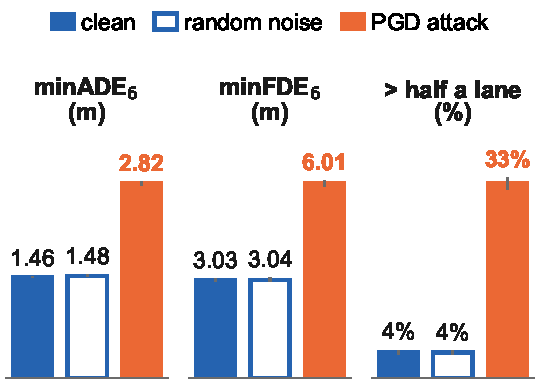
\includegraphics[width=\linewidth]{figures/results_final.pdf}
						{\centering\scriptsize Final model, 500 validation samples, mean of 3 seeds\par}
						\end{minipage}\hfill
						\begin{minipage}[c]{0.57\linewidth}
							\begin{itemize}
								\item \textbf{Yes:} PGD doubles both errors (minADE$_6$ $\times$1.93, minFDE$_6$ $\times$1.99) and 33\% of forecasts cross half a lane (4\% clean)
								\item \textbf{Direction, not noise:} same-size random noise (0.18\,m per point) changes nothing
								\item Zhang et al.~\cite{zhang2022adversarial}, averaged over their models and datasets: +167\%/+150\% ADE/FDE, 62\% past half a lane; ours +93\%/+99\%, 33\%
							\end{itemize}
						\end{minipage}
						\end{myblock}\vfill
						\begin{myblock}{Results: which component adds robustness?}
						\vspace{-0.3cm}
						\begin{figure}
							\centering
							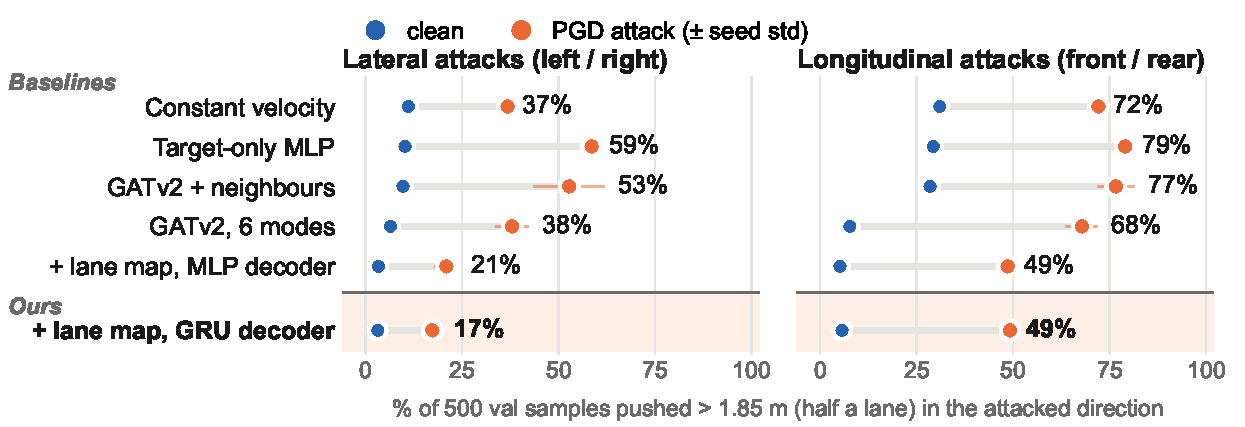
\includegraphics[width=\linewidth]{figures/results_models.pdf}
							\caption{Same 500 validation samples and 3 seeds for every model. The first three predict one future; the rest use the best of 6.}
						\end{figure}
						\begin{itemize}
							\item \textbf{The lane map helps most}, laterally: 38\%$\,\rightarrow\,$21\% past half a lane. Longitudinal attacks still reach 49\%
							\item \textbf{Neighbours and decoder barely matter:} GATv2 + neighbours vs target-only MLP: 53\% vs 59\% laterally, 77\% vs 79\% longitudinally; most GATv2 runs ignore their neighbours. GRU vs MLP decoder: 17\% vs 21\% and 49\% vs 49\%
						\end{itemize}
					\end{myblock}\vfill
					\begin{myblock}{Conclusions}
						\begin{itemize}
							\item 18\,cm of crafted, physically feasible driving pushes a third of our final model's forecasts more than half a lane off.
							\item Context the attacker cannot move, the \textbf{lane map}, adds robustness.
							\item \textbf{Limitations:}
							\begin{itemize}
								\item White-box, single frame, 500 validation samples; 1.85\,m is only a proxy
								\item 16\% of real traces already break the physical bounds and mostly stay unperturbed
							\end{itemize}
							\item \textbf{Next steps:}
							\begin{itemize}
								\item Build a GNN predictor that genuinely learns from its neighbours
								\item Test whether an attack on one road user spreads through the graph to others' predictions
								\item Turn this into an evaluation framework for adversarial attacks on trajectory predictors
							\end{itemize}
						\end{itemize}
					\end{myblock}\vfill
		}\end{minipage}\end{beamercolorbox}
	\end{column}
\end{columns}
\end{frame}
\end{document}
